\section{Graph-Based States}
\label{sec:gr-state}

In this section we explain the graph representation of FAJ states. We assume
that some translator generates a graph for a given program given by $Prog$ in
the grammar described above. This graph contains the static structure of the
base-program $\overline{L}$, static structure of point-cuts and advice
$\overline{A}$, and some representation of run-time information, which is
initialised by the main expression $e$ on the continuation stack. We describe
these parts one by one.

\subsection{AFJ Program Graph}

\begin{figure}
	\begin{center}
		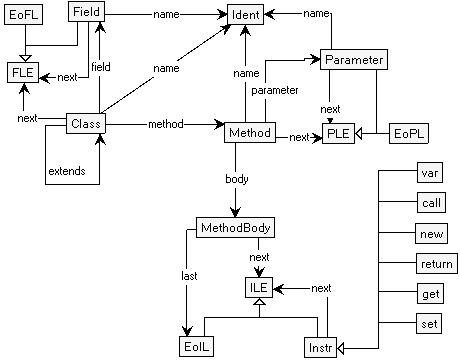
\includegraphics[scale=0.5]{other/static_meta.jpg}
	\end{center}
  \caption{Meta-Graph of the Base Language Static Structure}
	\label{fig:staticmeta}
\end{figure}

The static structure of the AFJ-part of the program (the base) is represented
by a graph conforming to the type-graph shown in Figure \ref{fig:staticmeta}.
Most of it should be self-explanatory. Classes have fields and methods. Methods
have parameters and a method body. A method body has a list of instructions.
Classes, fields, methods, and parameters have names. Fields, parameters, and
instructions are ordered in a list by \nextL-edges. The last element of a
list is an EoL node. List elements and EoL nodes can be either for fields (FLE,EoFL), parameters (PLE,EoPL) and instructions (ILE, EoIL).

The main expression --- not in this figure --- is on the
continuation stack, which is described shortly. Since type-checking is
neglected, return types, field types, and parameter types are not used and
therefore not represented in the graph.

\subsection{Aspect Program Graph}

\begin{figure}
	\begin{center}
		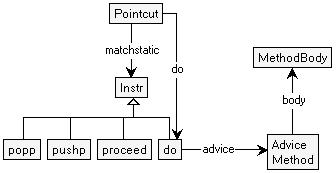
\includegraphics[scale=0.5]{other/aspect_meta.jpg}
	\end{center}
		\caption{Meta-Graph of the Aspectual Static Structure}
	\label{fig:meta_aspect}
\end{figure}

Advice is represented conforming to the meta-graph shown in Figure \ref{fig:meta_aspect}. Advice is modelled as a method, inheriting all options of regular methods. However, the body of an advice that can contain a {\sc proceed} instructions, where regular method cannot. Point-cuts are connected to all instructions they match. A point-cut is associated with an advice through a {\sc do} instruction, that is used to invoke the advice. 

\subsection{Run-time Graph}

Run-time information is represented conforming to the heap and stack
meta-graph, which is shown in Figure \ref{fig:runtime_meta}.  The heap is
represented as Objects that exist in the graph. Objects are connected to their
types. Values of fields are stored in the object as variables; the values
themselves are again Objects.  For method execution, a scope is created that
has variables for storing the values of the parameters. Instructions of the
method body on the continuation stack are also connected to the scope, such
that a {\sc var} instruction can find the correct value.

\begin{figure*}
	\begin{center}
		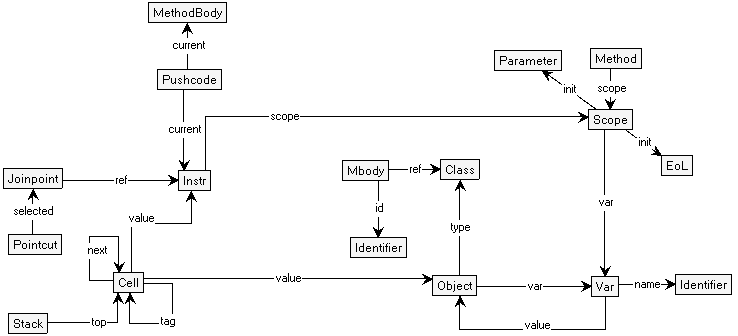
\includegraphics[scale=0.5]{other/runtime_meta.png}
	\end{center}
		\caption{Meta-graph of run-time information.}
	\label{fig:runtime_meta}
\end{figure*}

Execution is modelled as interpretation of instructions on the continuation
stack, and using values from a value stack. Therefore, most rules of the
semantics described in this paper perform one or more pop or push operations.
Stacks consists of a sequence of cells, the top one directly linked to the
stack itself. Cells can contain either instructions or objects. A cell can be
tagged, meaning that if this cell contains an instruction, this instruction
cannot trigger an advice. Stacks are named as follows: \emph{C} represents the
continuation stack, \emph{S} the value stack, \emph{P} the proceed stack.

Some auxiliary nodes can be created during execution that trigger and store
information for certain sub-routines. For example, the {\tt Mbody} is used for
method lookup, and the {\tt pushcode} node is used for pushing the instructions
of a method body on the continuation stack. Auxiliary instructions {\sc pushp}
and {\sc popp} can be created during advice execution.

\begin{comment}
We have chosen a graph based stack representation that allows pushing and popping uniformly, regardless of the stack containing one or more elements. This is shown in Figure \ref{fig:stack}. The left hand side left stack is an example of an empty stack, the right a stack with one element. The stack always has at least one {\tt Cell}. A pop operation is done by removing the top cell and create a new top edge to the new Cell on top of the stack. Would we model an empty stack as stack without the one (empty) cell, it would not be possible perform a pop like this when only one element is left on the stack. A rule for the pop operation is shown in figure \ref{fig:stack_pop}. The {\tt top} element of the Stack is removed from the stack (in this case removed from the graph), and a new {\tt top} edge is added to the new {\tt Cell} on top. When we say an element is popped from a stack, we mean that the {\tt top} edge of a stack is redirected to the {\tt Cell} below the current top of the stack. 

\begin{figure}
	\begin{center}
		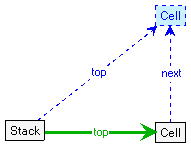
\includegraphics[scale=0.5]{other/stack_pop_example.png}
	\end{center}
		\caption{Stack pop operation}
	\label{fig:stack_pop}
\end{figure}
\end{comment}
